\documentclass{article}
\usepackage{amsmath}
\usepackage{amssymb}
\usepackage{amsfonts}
\usepackage{hyperref}
\usepackage{algpseudocode}
\usepackage{algorithm}
\usepackage{graphicx}


\title{Score-Based Generative Modeling Through Stochastic Differential Equations}
\author{Gaëtan Ecrepont, Samson Gourevitch, Logan Renaud}
\date{\today}

\begin{document}

\maketitle

\tableofcontents

\newpage

\section{Introduction and contribution} \label{sec:intro}
In 2020, Song et al. introduced a novel generative modeling framework \cite{score-matching} where samples are produced 
via Langevin dynamics using gradients from the data distribution. The gradients themselves are estimated using a technique known as denoising score matching, which was introduced in back in 2011 by Vincent \cite{score-da}. Six months after introducing this new generative model, Song et al. proposed a generalization under the lens of stochastic differential equations.
In this paper, we will first present Song et. al's first paper \cite{score-matching} in Section \ref{sec:score}, 
then in Section \ref{sec:sde} we will show how their second paper \cite{scorebased-sde} generalizes the first one. 
We will finally present the experiments and results in Section \ref{sec:experiments}.

Our contribution begins by summarizing and connecting the three aforementioned papers. 
Building on the work of Song et al., we will construct a neural network (the score network $s_\theta(\mathbf{x},t)$) 
from scratch and train it on the MNIST dataset. Using this score network, we will implement various sampling methods 
as described in Song et al.'s paper. We will then extend these methods to controlled generation, focusing on two types: conditional generation and inpainting.

\section{Estimating the score to sample data} \label{sec:score}
Generative modeling is the task of learning an unknown distribution $p_\text{data}(\mathbf{x})$ from a dataset 
$\mathcal{D} = \{\mathbf{x}_i\}_{i=1}^N \in (\mathbb{R}^d)^N$ of i.i.d. samples. The goal is to learn a generative model $p_\theta(\mathbf{x})$ 
such that $p_\theta(\mathbf{x}) \approx p_\text{data}(\mathbf{x})$. There are many ways to approach this problem. Perhaps the 
most natural way is to find $\theta$ that minimizes the Kullback-Leibler divergence between $p_\theta(\mathbf{x})$ and 
$p_\text{data}(\mathbf{x})$. It can be shown that this approach is equivalent to maximum likelihood estimation \cite{lyu}. 
However, it is intractable because the true data distribution is unknown. Instead, one can try to minimize the Fisher 
divergence between the two distributions. This is the approach taken by Song et al. and yields score-based generative modeling.

\subsection{Denoising score matching}

Given two distributions $p(\mathbf{x})$ and $q(\mathbf{x})$, the Fisher divergence is defined as
\begin{equation}
    D_F(p, q) = \mathbb{E}_{p(\mathbf{x})} \left[ \left\| \nabla_\mathbf{x} \log p(\mathbf{x}) - \nabla_\mathbf{x} \log q(\mathbf{x}) \right\|^2 \right].
\end{equation}

Contrary to the usual definition from statistics, here the score is the gradient of the log-density of the distribution 
with respect to the data $\mathbf{x}$ and not the parameters $\theta$. Intuitively, the score is a vector field that points
in the direction of the steepest ascent of the density i.e. towards "high probability" regions. To learn the score from 
the data, we can train a score network $\mathbf{s}_\theta: \mathbb{R}^d \to \mathbb{R}^d$ which minimizes the Fisher 
divergence with the true score $\nabla_\mathbf{x} \log p_\text{data}(\mathbf{x})$, i.e.
\begin{equation}
    \label{eq:score-naive}
    J^\text{naive}(\theta) = \frac{1}{2}\mathbb{E}_{p_\text{data}(\mathbf{x})} \left[ \left\| \mathbf{s}_\theta(\mathbf{x}) - \nabla_\mathbf{x} \log p_\text{data}(\mathbf{x}) \right\|^2 \right].
\end{equation}

However, this objective is intractable as is since the true score is unknown.
\footnote{Besides, Song et al. argue that approximating the true score is not a good idea 
for two reasons. First, since the data distribution is likely supported on a low-dimensional manifold (manifold hypothesis), the true score is likely to be undefined 
in the ambient space. Second, since there is little data in low-density region (i.e. far from the manifold), score estimation in these region is likely do be poor 
and that will negatively impact the sampling process, in particular because of the need to traverse low density regions to transition between modes of the data distribution.}
Instead, Song et al. propose to use denoising score matching, a technique introduced by Vincent in 2011 \cite{score-da}. In his paper, Vincent showed that under weak
regularity conditions, the objective $J^\text{naive}(\theta)$ is equivalent to
\begin{equation}
    \label{eq:score-denoising}
    J^\text{denoising}(\theta) = \frac{1}{2} \mathbb{E}_{\mathbf{x}\sim p_\text{data}(\mathbf{x}),\tilde {\mathbf{x}}\sim q_\sigma(\tilde {\mathbf{x}}|\mathbf{x})} \left[ \left\| \mathbf{s}_\theta(\tilde {\mathbf{x}}) - \nabla_{\tilde{ \mathbf{x}}} \log q_\sigma(\tilde {\mathbf{x}}|\mathbf{x}) \right\|^2 \right].
\end{equation}
where $\tilde {\mathbf{x}}\sim q_\sigma(\tilde {\mathbf{x}}|\mathbf{x})$ is a corrupted version of $\mathbf{x}$ and $q_\sigma(\tilde {\mathbf{x}}|\mathbf{x})$ is a noise distribution. 
The intuition behind this objective is that, given a noisy version of the data, the score network should point towards 
the original data point. Indeed, if we take an isotropic Gaussian noise distribution for $q_\sigma(\tilde {\mathbf{x}}|\mathbf{x})$,
we find that $\nabla_{\tilde {\mathbf{x}}} \log q_\sigma(\tilde {\mathbf{x}}|\mathbf{x}) = \frac{\mathbf{x} - \tilde {\mathbf{x}}}{\sigma^2}$, such that 
the score network is trained to point towards the original data point, i.e., to denoise the data.

\subsection{Training the score network}
Using our dataset $\mathcal{D}$, and selecting a noise distribution $q_\sigma(\tilde {\mathbf{x}}|\mathbf{x}) = \mathcal{N}(\tilde {\mathbf{x}}|\mathbf{x}, \sigma^2 \mathbf{I})$,
we can train the score network by minimizing the denoising score matching objective
\begin{equation}
    \label{eq:score-empirical}
    \ell(\theta; \sigma) = \frac{1}{2} \mathbb{E}_{\mathbf{x}\sim \mathcal{D}} \left[ \mathbb{E}_{\tilde {\mathbf{x}}\sim \mathcal{N}(\tilde {\mathbf{x}}|\mathbf{x}, \sigma^2 \mathbf{I})} \left[ \left\| \mathbf{s}_\theta(\tilde {\mathbf{x}}) - \frac{\mathbf{x} - \tilde {\mathbf{x}}}{\sigma^2} \right\|^2 \right] \right].
\end{equation}
The only question that remains is which $\sigma$ to choose. Using a small $\sigma$ will make the score target $\nabla_{\tilde {\mathbf{x}}} \log q_\sigma(\tilde {\mathbf{x}}|\mathbf{x})$
closer to the true score, but it will also bring back the issue that the true score is undefined in low-density regions. On the other hand, using a large $\sigma$ will make the
score target more regular across the ambient space. Song et al. propose to use a schedule for $\sigma$ that starts with a large value and decreases over time. Intuitively, this 
is a good idea because the high noise level will first help the Langevin dynamics to explore the data distribution and traverse low density regions, and then as we get closer to 
a mode, the noise level will decrease to help the Langevin dynamics converge to a point on the manifold, i.e. a realisitic sample.
Several schedules can be used. Song et al. propose a geometric sequence $\left \{ \sigma_t \right \}_{t=1}^T$ with $\sigma_t = \sigma_0 \gamma^t$ where $\sigma_0$ is the initial 
noise level, $\gamma$ is the decay rate, and $T$ is the number of noise levels.
The score network must thus be conditioned on the noise level $\sigma$ during training and inference, such that
\begin{equation}
    \forall \sigma \in \left \{ \sigma_t \right \}_{t=1}^T, \quad \mathbf{s}_\theta(\tilde {\mathbf{x}}; \sigma) \approx \nabla_{\tilde {\mathbf{x}}} \log q_\sigma(\tilde {\mathbf{x}}|\mathbf{x}).
\end{equation}
For the architecture, Song et al. propose to U-Net with conditional instance normalization layers
\footnote{If $\mathbf{x}$ is an input with $C$ feature maps, and we denote $\mu_k, \sigma_k$ the mean and standard deviation of the $k$-th feature map, conditional instance 
normalization with noise level $\sigma_i$ is achieved by setting $z_k = \gamma_{i,k} \frac{x_k - \mu_k}{\sigma_k} + \beta_{i,k}$ where $\gamma_{i,k}, \beta_{i,k}$ are
learnable parameters.}
to condition the score network on the noise level.

Finally, we can define our overall objective as a weighted sum of the denoising score matching objectives $\ell(\theta; \sigma_t)$ for all noise levels $\sigma_t$ in the schedule.
Here Song et al. proposes weighting $\lambda(\sigma) = \sigma^2$ such that $\lambda(\sigma)\ell(\theta; \sigma)=\frac{1}{2}\mathbb{E} \left[ \left\| \sigma\mathbf{s}_\theta(\tilde {\mathbf{x}}) - \frac{\mathbf{x} - \tilde {\mathbf{x}}}{\sigma} \right\|^2 \right]$
where $\frac{\mathbf{x} - \tilde {\mathbf{x}}}{\sigma} \sim \mathcal{N}(0, \mathbf{I})$ and $\| \sigma \mathbf{s}_\theta(\tilde {\mathbf{x}}) \|_2 \propto1$ such that the order
of magnitude of each term $\lambda(\sigma)\ell(\theta; \sigma)$ does not depend on $\sigma$.
We thus get the unified objective
\begin{equation}
    \label{eq:score-unified}
    \mathcal{L}(\theta, \left \{ \sigma_t\right \} _{t=1}^T) = \frac{1}{T} \sum_{t=1}^T \lambda(\sigma_t) \ell(\theta; \sigma_t).
\end{equation}
This objective can now be minimized with any flavor of stochastic gradient descent.

\subsection{Sampling with annealed Langevin dynamics}
Now that we have a trained score network, we can use Langevin dynamics, a type of Markov chain Monte Carlo (MCMC) method, to sample from the data distribution.
Given a fixed step size $\epsilon>0$ and an initial value $\tilde {\mathbf{x}}_0 \sim \pi(\mathbf{x})$ where $\pi$ is a tractable prior distrbution (e.g. a Gaussian), the Langevin
method recursively computes
\begin{equation}
    \tilde {\mathbf{x}}_{t} = \tilde {\mathbf{x}}_{t-1} + \frac{\epsilon}{2} \nabla_\mathbf{x} \log p(\tilde {\mathbf{x}}_{t-1}) + \sqrt{\epsilon}\mathbf{z}_t
\end{equation}
where $\mathbf{z}_t \sim \mathcal{N}(0, \mathbf{I})$. The distrbution of $\tilde {\mathbf{x}}_T$ converges to the data distribution $p(\mathbf{x})$ as $\epsilon \to 0$ and $T \to \infty$.
In practice, $\epsilon>0$ and $T<\infty$, which creates an error in the sampling process, but we can assume that this error is small enough to be ignored.

In practice, since we have different noise levels $\sigma_t$ in the schedule, we use annealed Langevin dynamics. More details in \ref{subsec:langevin}.


\section{Reverting SDEs to sample data} \label{sec:sde}

\subsection{Sampling using reverse SDEs instead of Langevin dynamics}
The Langevin dynamics method presented above works well in practice and scales up nicely to higher dimensions. In effect, we have learned how to gradually noise and gradually 
denoise our data, through discrete noise levels $\sigma_t$ in the schedule.
However, Song et al. found six months later that this discrete noising process could be subsumed into a continous-time stochastic differential equation (SDE) framework. This is
very interesting because we know from Anderson \cite{anderson} that the reverse of a diffusion process is also a diffusion process. Indeed, given a diffusion process
\begin{equation}
    d\mathbf{x}_t = \mathbf{f}(\mathbf{x}_t,t)dt + g(t)d\mathbf{w}_t
\end{equation}
the reverse process is
\begin{equation}
    d\mathbf{x}_t = \left[ \mathbf{f}(\mathbf{x}_t,t) - g(t)^2 \nabla_\mathbf{x} \log p_t(\mathbf{x}_t) \right]dt + d\mathbf{\bar{w}}_t
\end{equation}
where $p_t(\mathbf{x})$ is the density of the process at time $t$ (which is given by the Fokker-Planck equation) and $\mathbf{\bar{w}}_t$ is a Wiener process when time flows backwards from $T$ to $0$.
Thus, by starting from $\mathbf{x}_T \sim p_T(\mathbf{x})$ and running the reverse process, we can obtains samples $\mathbf{x}_0 \sim p_0(\mathbf{x})$.
Therefore, instead of using Langevin dynamics to sample from $p_\text{data}(\mathbf{x})$, we can use the reverse of the diffusion process. This is the idea behind the SDE-based generative model.

\subsection{Adapting the score network}
The only modification needed is to make our score network conditional on the continuous time $t$ instead of the discrete noise level $\sigma_t$ we previously used. The most natural 
way to to achieve this time-conditioning is to give $t$ as an input to the score network with a learnable time embedding on each layer of the U-Net. The error we try to minimize to train 
the score network thus becomes
\begin{equation}
    \label{eq:score-sde}
    \mathcal{L}(\theta) = \mathbb{E}_t \left[ \lambda(t) \mathbb{E}_{\mathbf{x}(0)} \left[ \mathbb{E}_{\mathbf{x}(t)| \mathbf{x}(0)} \left[ \left\| \mathbf{s}_\theta(\mathbf{x}(t), t) - \nabla_{\mathbf{x}(t)} \log p_{0t}(\mathbf{x}(t)|\mathbf{x}(0)) \right\|^2 \right] \right] \right]
\end{equation}
where $\lambda : [0,T] \to \mathbb{R}_+^*$ is a weighting function, $t\sim \mathcal{U}(0,T)$, $\mathbf{x}(0) \sim p_0(\mathbf{x})$, and 
$\mathbf{x}(t) \sim p_{0t}(\mathbf{x}(t)|\mathbf{x}(0))$ where $p_{st}(\mathbf{x}(t)|\mathbf{x}(s))$ denotes the transition kernel of the diffusion process from time $s$ to time $t>s$.
\footnote{That is, we have $p_t(\mathbf{x}(t)) = \int p_{st}(\mathbf{x}(t)|\mathbf{x}(s))p_s(\mathbf{x}(s))ds$.}

\subsection{Link with the discrete noising process from Section \ref{sec:score}}
Note that in Section \ref{sec:score}, we used gaussian perturbation kernels such that $q_\sigma(\tilde {\mathbf{x}}|\mathbf{x}) = \mathcal{N}(\tilde {\mathbf{x}}|\mathbf{x}, \sigma^2 \mathbf{I})$.
This corresponds to the following Markov chain:
\begin{equation}
    \mathbf{x}_t = \mathbf{x}_{t-1} + \sqrt{\sigma_i^2 - \sigma_{i-1}^2} \mathbf{z}_{t-1} \quad t = 1, \ldots, T
\end{equation}
In the limit $T \to \infty$, $\left \{ \sigma_t \right \}_{t=1}^T$ becomes $\sigma(t)$, $\mathbf{z}_t$ becomes $d\mathbf{w}_t$, and the Markov chain $\left \{ \mathbf{x}_t \right \}_{t=1}^T$ becomes 
the process $\left \{ \mathbf{x}(t) \right \}_{t\in[0,1]}$ given by the following SDE:
\footnote{Likewise, the noising schedule proposed by Ho et al. in \cite{ho} can be seen as a discretization of another SDE.}
\begin{equation}
    d\mathbf{x}(t) = \sqrt{\frac{d\sigma^2(t)}{dt}} d\mathbf{w}(t)
\end{equation}

\subsection{Sampling using ODE}
There is another way to sample from the data distribution using the SDE-based generative model. It hinges on this remarkable fact: for all diffusion processes 
$d\mathbf{x}(t) = \mathbf{f}(\mathbf{x}(t),t)dt + g(t)d\mathbf{w}(t)$, there exists a corresponding deterministic process whose trajectories share the same marginal 
(but not joint) probability densities $\left \{ p_t(\mathbf{x}) \right \}_{t\in[0,T]}$.
This deterministic process satisfies the ordinary differential equation (ODE)
\begin{equation}
    d\mathbf{x}(t) = \left[ \mathbf{f}(\mathbf{x}(t), t) - \frac{1}{2}g(t)^2 \nabla_\mathbf{x} \log p_t(\mathbf{x}(t)) \right] dt
\end{equation}
We can thus sample from the data distribution by solving the ODE from time $T$ to time $0$ starting from $\mathbf{x}(T) \sim p_T(\mathbf{x})$. This approach has many advantages:
it allows for fast sampling with black-box ODE solvers, it allows for exact likelihood computation, and it allows for latent space manipulation (e.g. interpolation).

\subsection{Predictor-Corrector Sampling}
So far we have introduced three ways to sample from the data distribution: Langevin dynamics, reverse SDEs, and ODEs.
Reverse SDEs and ODEs are linked and both use the idea of going back in time to revert the diffusion process. But unlike generic SDEs, here we have additional
information which we can use to improve the sampling process: indeed, we have an approximation of the score $\mathbf{s}_\theta(\mathbf{x}, t)$ at each time $t$.
This allows us to use MCMC sampling to "correct" the reverse diffusion process obtained from the SDE or the ODE. This is the idea behind the predictor-corrector sampling method,
which at each step combines a prediction step (using the reverse SDE or the ODE) and a correction step (using Langevin dynamics). Empirically, this method yields superior results 
compared to using predictor only or corrector only.

\section{Controllable generation}
So far, we have described several methods for generating random samples from the data distribution. However, the diffusion approach is flexible and can easily be tweaked to control the generation process. The idea is the following: if we denote by $\mathbf{y}$ the conditions we want to impose on the generated samples, we aim to sample from the conditional distribution \( p_\text{data}(\mathbf{x}|\mathbf{y}) \). Starting with random noise, we reverse through time by following either the reverse SDE or the probability flow ODE, adjusting the process to use \( \nabla_\mathbf{x} \log p_t(\mathbf{y}|\mathbf{x}) \) instead of \( \nabla_\mathbf{x} \log p_t(\mathbf{x}) \). Intuitively, this approach reverts the diffusion of $\{ \mathbf{x}_t|\mathbf{y}\}_{t\in[0,T]}$
\footnote{Note that this is not a formal definition but conveys the idea that $\mathbf{x}$'s diffusion process is not the same when we condition on $\mathbf{y}$.}
instead of $\{ \mathbf{x}_t\}_{t\in[0,T]}$, meaning our final sample will satisfy \( \mathbf{x}_0 \sim p_0(\mathbf{x}|\mathbf{y}) \) as desired.

To illustrate, we implemented this heuristic in two key applications: class-conditional generation and inpainting.


\subsection{Class-conditional generation}
Let's assume that each data point $\mathbf{x}$ is associated with a label $\mathbf{y}$. We want to condition the generation process of $\mathbf{x}$ on the label $\mathbf{y}$.
If we consider again the diffusion SDE $d\mathbf{x}=f(\mathbf{x},t)dt+g(t)d\mathbf{w}$ \textit{and} we assume that the initial distribution is $p_0(\mathbf{x}|\mathbf{y})$,
then again using \cite{anderson} we can show that the reverse of the diffusion process is given by $d\mathbf{x}=[f(\mathbf{x},t)-g(t)^2\nabla_\mathbf{x}\log p_t(\mathbf{x}|\mathbf{y})]dt+d\mathbf{\bar{w}}$.
And remarking that $\nabla_\mathbf{x}\log p_t(\mathbf{x}|\mathbf{y})=\nabla_\mathbf{x}\log p_t(\mathbf{x})+\nabla_\mathbf{x}\log p_t(\mathbf{y}|\mathbf{x})$, we obtain the conditional reverse SDE
\begin{equation}
    d\mathbf{x}=[f(\mathbf{x},t)-g(t)^2\left(\nabla_\mathbf{x}\log p_t(\mathbf{x}) + \nabla_\mathbf{x}\log p_t(\mathbf{y}|\mathbf{x}) \right)]dt+g(t)d\mathbf{\bar{w}}
\end{equation}
It is easy to approximate $\nabla_\mathbf{x}\log p_t(\mathbf{y}|\mathbf{x})$ by training a classifier which learns to predict the label $\mathbf{y}$ from the data $\mathbf{x}$, and then performing
backpropagation to obtain the gradient of the log-likelihood of the label given the data.

\subsection{Imputation} \label{subsec:imputation}
Imputation corresponds to the task of filling in missing values in a data point $\mathbf{x}$ sampled from the data distribution $p_\text{data}(\mathbf{x})$.
We can use the same idea as for class-conditional generation: if we denote $\Omega(\mathbf{x})$ and $\bar{\Omega}(\mathbf{x})$ the observed and missing dimensions of $\mathbf{x}$ respectively,
then we can consider the missing part $\mathbf{z}=\bar{\Omega}(\mathbf{x})$ as a latent variable which follows its own diffusion process $d\mathbf{z}=f_{\bar{\Omega}}(\mathbf{z},t)dt+g(t)d\mathbf{w}_{\bar{\Omega}}$
where we have restricted the dynamics to the missing dimensions.
Then, we want to condition this diffusion based on the observed part $\Omega(\mathbf{x}(0))$, and then reverse this conditional diffusion process to sample the missing part $\mathbf{z}(0)$.
Using \cite{anderson} again, we obtain the reverse SDE conditioned on $\Omega(\mathbf{x}(0))=\mathbf{y}$:
\begin{equation}
    d\mathbf{z}=[f_{\bar{\Omega}}(\mathbf{z},t)-g(t)^2\nabla_\mathbf{z}\log p_t(\mathbf{z}|\Omega(\mathbf{x}))]dt+d\mathbf{\bar{w}}_{\bar{\Omega}}
\end{equation}
Here we are stuck because $p_t(\mathbf{z}|\Omega(\mathbf{x}))$ is intractable in general. It can however be approximated by $p_t(\mathbf{z}|\hat{\Omega}(\mathbf{x}))$
where $\hat{\Omega}(\mathbf{x})$ is a random sample from $p_t(\Omega(\mathbf{x}(t))|\Omega(\mathbf{x}(0))=\mathbf{y})$. We thus obtain
$\nabla_\mathbf{z}\log p_t(\mathbf{z}|\Omega(\mathbf{x}(0)=\mathbf{y}))\approx\nabla_\mathbf{z}\log p_t(\mathbf{z}|\hat{\Omega}(\mathbf{x}))=\nabla_\mathbf{z}\log p_t(\left[ \mathbf{z}, \hat{\Omega}(\mathbf{x}) \right])$
where we have concatenated the missing part $\mathbf{z}$ with the observed part $\hat{\Omega}(\mathbf{x})$ but we are still taking the gradient only with respect to $\mathbf{z}$ only.

\section{Experiments and results} \label{sec:experiments}
In this section we will implement all the sampling methods detailed above on the MNIST dataset, which we chose because it hasn't been used in the original paper, and also 
because of the lower computational cost compared to other higher dimensional datasets like CIFAR-10 or CelebA. We will not compute evaluation metrics like the inception score or the FID score since
this has already been done in the original papers, but we will give qualitative comments.

\subsection{Annealed Langevin dynamics} \label{subsec:langevin}
\begin{algorithm}[H]
	\caption{Annealed Langevin dynamics}
	\label{alg:anneal}
	\begin{algorithmic}[1]
	    \Require{$\{\sigma_i\}_{i=1}^L, \epsilon, T$.}
	    \State{Initialize $\tilde{\mathbf{x}}_0 \sim \mathcal{N}(0, \sigma_1^2 I)$.}
	    \For{$i \gets 1$ to $L$}
	        \State{$\alpha_i \gets \epsilon \cdot \sigma_i^2/\sigma_L^2$} \Comment{$\alpha_i$ is the step size.}
            \For{$t \gets 1$ to $T$}
                \State{Draw $\mathbf{z}_t \sim \mathcal{N}(0, I)$}
                \State{$\tilde{\mathbf{x}}_{t} \gets \tilde{\mathbf{x}}_{t-1} + \dfrac{\alpha_i}{2} \, \mathbf{s}_\theta(\tilde{\mathbf{x}}_{t-1}, \sigma_i) + \sqrt{\alpha_i} \, \mathbf{z}_t$}
            \EndFor
            \State{$\tilde{\mathbf{x}}_0 \gets \tilde{\mathbf{x}}_T$}
        \EndFor
        \item[]
        \Return{$\tilde{\mathbf{x}}_T$}
	\end{algorithmic}
\end{algorithm}
In practice, we use step size $\alpha_i \propto \sigma_i^2$ is to keep the signal-to-noise ratio $\frac{ \alpha_i s_\theta(\tilde {\mathbf{x}}, \sigma_i)}{2\sqrt{\alpha_i}\mathbf{z}}$ constant across noise levels.

\begin{figure}[H]
    \centering
    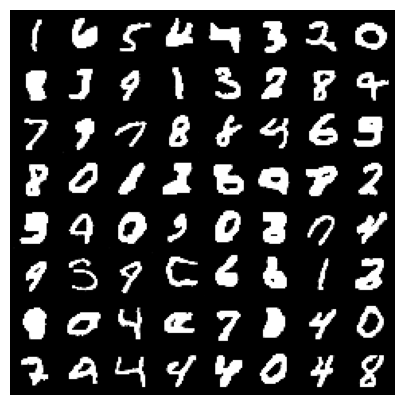
\includegraphics[width=0.5\textwidth]{images/langevin.png}
    \caption{Samples generated using annealed Langevin dynamics.}
    \label{fig:langevin}
\end{figure}
The samples generated are diverse and of decent quality, but the digits are not as sharp as we would like them to be.
Hyperparameter search on $L, \epsilon, T$ did not significantly improve the results, indicating that the issue probably lies in the score network,
which we have only trained for 5 epochs due to computational constraints.

\subsection{Reverse SDE}
We use the Euler-Maruyama method to solve the reverse SDE.
\begin{algorithm}[H]
	\caption{Euler-Maruyama method for reverse SDE}
	\label{alg:reverse-sde}
	\begin{algorithmic}[1]
	    \Require{$\sigma, N, T$.}
	    \State{Initialize $\tilde{\mathbf{x}}_N \sim \mathcal{N}(0, \int_0^T \sigma^2(t)dt I)$.}
        \State{$\Delta t \gets T/N$}
	    \For{$k \gets N$ to $1$}
            \State{Draw $\mathbf{z}_k \sim \mathcal{N}(0, I)$}
            \State{$t \gets k \cdot \Delta t$}
            \State{$\tilde{\mathbf{x}}_{k-1}^\text{mean} = \tilde{\mathbf{x}}_{k} + \sigma^2(t) \mathbf{s}_\theta(\tilde{\mathbf{x}}_{k}, t) \Delta t$}
            \State{$\tilde{\mathbf{x}}_{k-1} \gets \tilde{\mathbf{x}}_{k-1}^\text{mean} + \sigma(t) \sqrt{\Delta t} \mathbf{z}_k$}
        \EndFor
        \item[]
        \Return{$\tilde{\mathbf{x}}_0^\text{mean}$}
	\end{algorithmic}
\end{algorithm}

\begin{figure}[H]
    \centering
    \includegraphics[width=0.5\textwidth]{images/sde.png}
    \caption{Samples generated using reverse SDE.}
    \label{fig:sde}
\end{figure}

Using the reverse SDE, we obtain sharper samples than with Langevin dynamics, as expected. The diversity is still good.

\subsection{ODE}
We simply feed the initial value $\tilde{\mathbf{x}}_T \sim \mathcal{N}(0, \int_0^T \sigma^2(t)dt I)$ and the ODE $d\mathbf{x} = -\frac{1}{2}g(t)^2 s_\theta(\mathbf{x}, t)dt$ to a black-box ODE solver.

\begin{figure}[H]
    \centering
    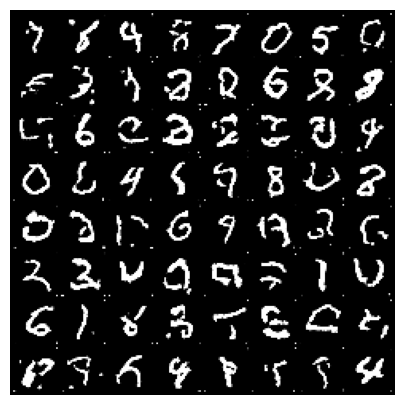
\includegraphics[width=0.5\textwidth]{images/ode.png}
    \caption{Samples generated using ODE.}
    \label{fig:ode}
\end{figure}

ODE allows for much faster sampling (only $\sim100$ iterations needed, vs. $\sim1000$ for Langevin dynamics and reverse SDE), but the samples are not realistic, although sharp.

\subsection{Predictor-Corrector Sampling}
We simply pick a predictor (reverse SDE or ODE) and a corrector (Langevin dynamics) and alternate between the two methods according to the following algorithm.
\begin{algorithm}[H]
	\caption{Predictor-Corrector Sampling}
	\label{alg:predictor-corrector}
	\begin{algorithmic}[1]
	    \Require{$\sigma, N, T$, predictor, corrector.}
	    \State{Initialize $\tilde{\mathbf{x}}_N \sim \mathcal{N}(0, \int_0^T \sigma^2(t)dt I)$.}
        \State{$\Delta t \gets T/N$}
	    \For{$k \gets N$ to $1$}
            \State{$\tilde{\mathbf{x}}_{k-1} \gets \text{corrector}(\tilde{\mathbf{x}}_k)$}
            \State{$\tilde{\mathbf{x}}_{k-1} \gets \text{predictor}(\tilde{\mathbf{x}}_{k-1})$}
        \EndFor
        \item[]
        \Return{$\tilde{\mathbf{x}}_0^\text{mean}$}
	\end{algorithmic}
\end{algorithm}

\begin{figure}[H]
    \centering
    \includegraphics[width=0.5\textwidth]{images/pc_sde.png}
    \caption{Samples generated using predictor-corrector sampling.}
    \label{fig:pc}
\end{figure}

As expected, predictor-corrector sampling yields the best results, with sharp, realistic and diverse samples.

\subsection{Class-conditional generation}
For class-conditional generation, we train a time-conditional Multi Layer Perceptron (MLP) to predict the label $\mathbf{y}$ from the noised data $\mathbf{x}(t)$.
We can then obtain $\nabla_\mathbf{x}\log p_t(\mathbf{y}|\mathbf{x})$ by backpropagation, which is easy in PyTorch using the autograd feature.
We can now use any sampling method detailed above to sample conditionally on the label $\mathbf{y}$, simply by replacing $\nabla_\mathbf{x}\log p_t(\mathbf{x})$ by $\nabla_\mathbf{x}\log p_t(\mathbf{x}) + \nabla_\mathbf{x}\log p_t(\mathbf{y}|\mathbf{x})$ in the algorithm.

\begin{figure}[H]
    \centering
    \includegraphics[width=0.5\textwidth]{images/cond.png}
    \caption{Samples generated using class-conditional generation with $\mathbf{y}=4$.}
    \label{fig:cond}
\end{figure}

The samples generated are all 4's as expected and they are of good quality.
Interestingly, SDE class-conditional sampling yields more realistic samples than vanilla SDE sampling.

\subsection{Imputation}
We use the method detailed in \ref{subsec:imputation} to generate samples conditionally on the observed part $\Omega(\mathbf{x})$. This does not require any additional training and is compatible with all the sampling methods detailed above.
Below is the algorithm if we use for instance the reverse SDE as the predictor and no corrector.
\begin{algorithm}[H]
	\caption{Imputation}
	\label{alg:imputation}
	\begin{algorithmic}[1]
	    \Require{$\sigma, N, T, \Omega(\mathbf{x})$.}
	    \State{Initialize $\tilde{\mathbf{z}}_N \sim \mathcal{N}(0, \int_0^T \sigma^2(t)dt I_{\bar{\Omega}}$.}
        \State{$\Delta t \gets T/N$}
	    \For{$k \gets N$ to $1$}
            \State{Draw $\mathbf{z}_k \sim \mathcal{N}(0, I_{\Omega})$}
            \State{$t \gets k \cdot \Delta t$}
            \State{$\hat{\Omega}(\mathbf{x}(t)) \gets \Omega(\mathbf{x}(0)) + \mathcal{N}(0, \int_0^t \sigma^2(t)dt I_{\Omega})$}
            \State{$\tilde{\mathbf{z}}_{k-1}^\text{mean} = \tilde{\mathbf{z}}_{k} + \sigma^2(t) \mathbf{s}_\theta(\left[ \tilde{\mathbf{z}}_{k}, \hat{\Omega}(\mathbf{x}) \right], t) \Delta t$}
            \State{$\tilde{\mathbf{z}}_{k-1} \gets \tilde{\mathbf{z}}_{k-1}^\text{mean} + \sigma(t) \sqrt{\Delta t} \mathbf{z}_k$}
        \EndFor
        \item[]
        \State{$\tilde{\mathbf{x}}_0 \gets \left[ \tilde{\mathbf{z}}_0, \Omega(\mathbf{x}(0)) \right]$}
        \item[]
        \Return{$\tilde{\mathbf{x}}_0$}
	\end{algorithmic}
\end{algorithm}

\begin{figure}[H]
    \centering
    \includegraphics[width=0.4\textwidth]{images/inpainting_noised.png}
    \includegraphics[width=0.4\textwidth]{images/inpainting_denoised.png}
    \caption{Left: masked MNIST samples. Right: after inpainting.}
    \label{fig:inpainting}
\end{figure}

The inpainting results are very good, with the missing parts filled in correctly, expect for 1s which end up completely wiped out by the middle vertical mask.
Other masks (e.g. middle horizontal or uniform with pixel-wise Bernoulli mask) yield satisfying results as well.

\newpage

\bibliographystyle{plain}
\begin{thebibliography}{9}

\bibitem{score-matching}
    Yang Song and Stefano Ermon. 
    \textit{Generative Modeling by Estimating Gradients of the Data Distribution}. 
    Advances in Neural Information Processing Systems 32 (NeurIPS), 2019.

\bibitem{scorebased-sde}
    Yang Song, Jascha Sohl-Dickstein, Diederik P. Kingma, Abhishek Kumar, Stefano Ermon, and Ben Poole.
    \textit{Score-Based Generative Modeling through Stochastic Differential Equations}. 
    arXiv preprint arXiv:2011.13456, 2021.

\bibitem{score-da}
    Pascal Vincent. 
    \textit{A Connection Between Score Matching and Denoising Autoencoders}. 
    Neural Computation, 23(7):1661–1674, 2011.

\bibitem{lyu}
    Lyu, S.
    \textit{Interpretation and generalization of score matching.}
    Proceedings of the 25th Conference in Uncertainty in Artificial Intelligence (UAI'09), 2010.

\bibitem{anderson}
    Anderson, B. D. O.
    \textit{Reverse-time diffusion equation models.}
    Stochastic Processes and their Applications, 12(3), 313–326, 1982.

\bibitem{ho}
    Ho, J., Jain, A., and Abbeel, P.
    \textit{Denoising Diffusion Probabilistic Models}
    Advances in Neural Information Processing Systems (NeurIPS), 33, 6840–6851, 2020.

\end{thebibliography}
\end{document}
